\section{Differenzierbarkeit}
\subsection{Definition}
$f$ ist in $a \in I$ differenzierbar mit der Ableitung $f'(a)$, wenn
\[
\lim_{x \to a} \frac{f(x) - f(a)}{x - a} =: f'(a) = \frac{d}{dx}f(a)
\]
existiert.

Ist $f'$ stetig im Definitionsbereich, so heisst $f$ stetig differenzierbar. Man
kann also $f$ differenzieren und bekommt mit $f'$ eine stetige Funktion. Es gilt
auch $f \in C^1(I)$. $C^n(I)$ ist die Menge der $n$-mal stetig differenzierbaren
Funktionen über dem Intervall $I$.

\subsection{Mittelwertsatz (Satz von Lagrange)}
Ist $f$ auf $[a,b]$ stetig und in $]a, b[$ differenzierbar, so gibt es ein $c
\in ]a,b[$ mit\\

% 2 columns (don't insert a new linew between minipage definition, otherwise the layout will break!)
% In order to place the text on top/middle of column next to the image \vspace{0pt} must be inserted!
% Otherwise the text will appear on bottom! Go figure..
\begin{minipage}{0.25\textwidth}
	\vspace{0pt}
	\[
	\frac{f(b) - f(a)}{b-a} = f'(c)
	\]
\end{minipage}
\begin{minipage}{0.25\textwidth}
		\vspace{0pt}
	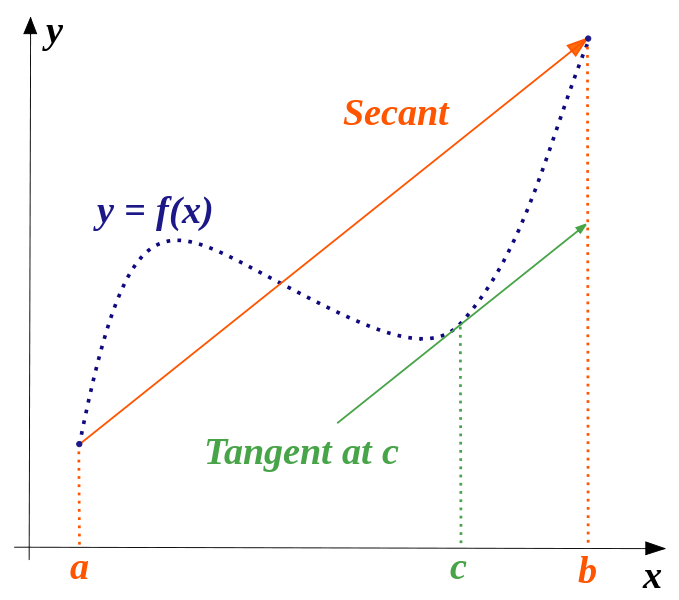
\includegraphics[scale=0.15]{mittelwertsatz.png}
\end{minipage}

\subsubsection{Beispiel: Ungleichungen}
Zu zeigen: $e^x(y-x) < e^y - e^x < e^y(y-x), \; \forall x < y$:


Der Mittelwertsatz wird auf die Exponentialfunktion angewendet. Damit gilt für
ein Paar von Zahlen $x < y$ ein $u \in ]x,y[$, für welches gilt: $\frac{e^y
- e^x}{y-x} = e^u$. Weil die Exponentialfunktion in $\R$ streng monoton wachsend
ist, gilt $e^x < e^u < e^y$ und somit gilt: $e^x < \frac{e^y-e^x}{y-x} < e^y$.
Multipliziert man nun mit dem Nenner des Bruchs bekommt man: $e^x (y-x) < e^y -
e^x < e^y(y-x)$.

\subsection{Monotonie}
\begin{itemize}
	\item $f' > 0 \Rightarrow f$ streng monoton steigend
	\item $f' \geq 0 \Leftrightarrow f$ monoton steigend
	\item $f' < 0 \Rightarrow f$ streng monoton fallend
	\item $f' \leq 0 \Leftrightarrow f$ monoton fallend
\end{itemize}
Insbesondere besitzt die Funktion $f$ wenn sie streng monoton wachsend/fallend ist
weder kritische Punkte, noch lokale oder globale Extrema.

\subsection{Konvexität}

\begin{definition}[konvex]
Eine Funktion $f: \Omega \to \R$ heisst konvex ($\cup$) , wenn $\forall x_1,x_2 \in \Omega$ und $t \in [0, 1]$ gilt:\\
$f(x_1 + t(x_2 - x_1)) \leq f(x) + t(f(x_2) - f(x_1))$
\end{definition}

\underline{Anschaulich:} Anschaulich bedeutet das, dass bei einer konvexen Funktion
der Graph immer unter der Sekante liegt. Der Graph konvexer Funktionen ist linksgekrümmt

\begin{itemize}
	\item $f'' \geq 0 \Leftrightarrow f$ konvex
\end{itemize}

\subsection{Extremstellen}
Extrema sind lokale und globale Maxima und Minima. 
\begin{itemize}
	\item Extrema bei $x_0 \Rightarrow f'(x_0) = 0$
	\item $f'(x_0) = 0, f''(x_0) > 0 \Rightarrow$ Minimum bei $x_0$
	\item $f'(x_0) = 0, f''(x_0) < 0 \Rightarrow$ Maximum bei $x_0$
	\item $f'(x_0) = 0, f''(x_0) = 0, f'''(x_0) \neq 0 \Rightarrow$ Sattelpunkt in $x_0$
	\item \hspace{1.6cm} $f''(x_0) = 0, f'''(x_0) \neq 0 \Rightarrow$ Wendepunkt in $x_0$
\end{itemize}
Merke: Jeder Sattelpunkt ist auch ein Wendepunkt!

\subsubsection{Beispiel Wendepunkt berechnen}
%Von http://www.frustfrei-lernen.de/mathematik/wendepunkt-berechnen.html
Die hinreichende Bedingung für einen Wendepunkt lautet: $f''(x_0) = 0$ und $f'''(x_0) \not= 0$\\
 
Praktische Vorgehensweise für $f(x) = \frac{1}{3}x^3-2x^2+3x$:\\
Um eine Funktion auf Wendepunkte hin zu untersuchen, führen wir die folgenden Schritte durch:
\begin{itemize}
	\item Wir leiten die Funktion f(x) dreimal ab. $f'(x) = x^2-4x+3$, $f''(x) = 2x-4$ und $f'''(x) = 2$
	\item Wir setzen die zweite Ableitung Null und berechnen den X-Wert, sofern möglich  
		$f''(x) = 2x-4 \stackrel{!}{=} 0 \Rightarrow x = 2$ 
	\item Sofern möglich, setzen wir diesen X-Wert in die dritte Ableitung ein
		$f'''(x) = 2$
	\item Ist dieses Ergebnis ungleich Null, liegt ein Wendepunkt vor
		$f'''(x) = 2 \not= 0 \Rightarrow$ Wendepunkt
	\item Der X-Wert wird in f(x) eingesetzt, um den zugehörigen Y-Wert zu bestimmen.
		$x = 2$ in $f(x)$ einsetzen: $f(2) = \frac{1}{3}2^3-2\cdot2^2+3\cdot2 = \frac{2}{3}$
\end{itemize}

\subsection{Zusammenhang zwischen Stetigkeit und Differenzierbarkeit}
\begin{itemize}
	\item differenzierbar $\Rightarrow$ stetig
	\item differenzierbar $\not\Leftarrow$ stetig
\end{itemize}

\subsection{Umkehrsatz}
% aus http://mathematik-netz.de/pdf/Umkehrsatz.pdf
Ist $f:I \to \R$ auf I differenzierbar mit $f'(x) \neq 0$ für jedes $x \in I$,
so ist $f$ streng monoton wachsend oder streng monoton fallend und damit
injektiv. Die Umkehrfunktion $f^{-1}:f(I) \to I$ existiert und ist ebenfalls
streng monoton wachsend oder streng monoton fallend. Die Ableitung
$(f^{-1})'(y)$ existiert für alle $y \in f(I)$ mit $f'(f^{-1}(y)) \neq 0)$, und zwar gilt dann \[ (f^{-1})'(y) = \frac{1}{f'(f^{-1}(y))}
\]

\subsection{Monotonie, Bijektion, Differenzierbarkeit}
\begin{satz}
(\textit{Folgendes gilt auch für streng monoton fallende Funktionen})

Sei $f: [a, b] \to \R$ stetig und streng monoton wachsend. Es sei dann
$A = f(a), B = f(b)$, dann gilt: $f: [a,b] \to [A, B]$ ist bijektiv.

$f$ hat also eine Umkehrfunktion $f^{-1}: [A,B] \to [a,b]$ und diese ist stetig
und streng monoton wachsend.
\end{satz}

\underline{Tipp:} Differentierbare Funktionen sind stetig.
